


\documentclass{article}
\usepackage{graphicx}
\usepackage{minted}
\usepackage{parskip}
\usepackage{hyperref}

\definecolor{bg}{rgb}{0.95, 0.95, 0.95}
\begin{document}
\section*{Evaluating and plotting functions with Matlab}

In this session, you will use Matlab as a fancy calculator. You will learn
to evaluate and graph functions, and apply this new-found ability to do some
\emph{real} science.

Let's use Matlab to evaluate a function, say $y = sin(x^{2})$, for some
$x$.

\begin{minted}[bgcolor=bg]{octave}
    >> x = 1.0;        
    >> y = sin(x^2);
    >> disp(y)
\end{minted}

But we can do more. We can evaluate $sin(x^2)$ for a series
of $x$.

\begin{minted}[bgcolor=bg]{octave}
    >> % Enclose a series within square brackets
    >> x = [-2 -1.5 -1 -0.5 0 0.5 1 1.5 2];
    >> y = sin(x.^2); % Evaluates y for each x
    >> disp(y)
\end{minted}

Take note of the dot (\texttt{.}) in \texttt{sin(x.\^{}2)}. Matlab will be
very unhappy if you forget it -- we'll talk about why soon. For now, just remember
this:

\begin{figure}[hc]
\fbox{\textbf{Put a \texttt{.} before every multiplication and exponentiation sign (\texttt{.*} and \texttt{.\^{}}) }}
\end{figure}

With a bunch of numbers \texttt{x} and the corresponding values of 
\texttt{y = sin(x$^2$)}, we are in a position to \emph{graph} our function:

\begin{minted}[bgcolor=bg]{octave}
    >> plot(x, y)
\end{minted}

\begin{figure}[h]
\begin{center}
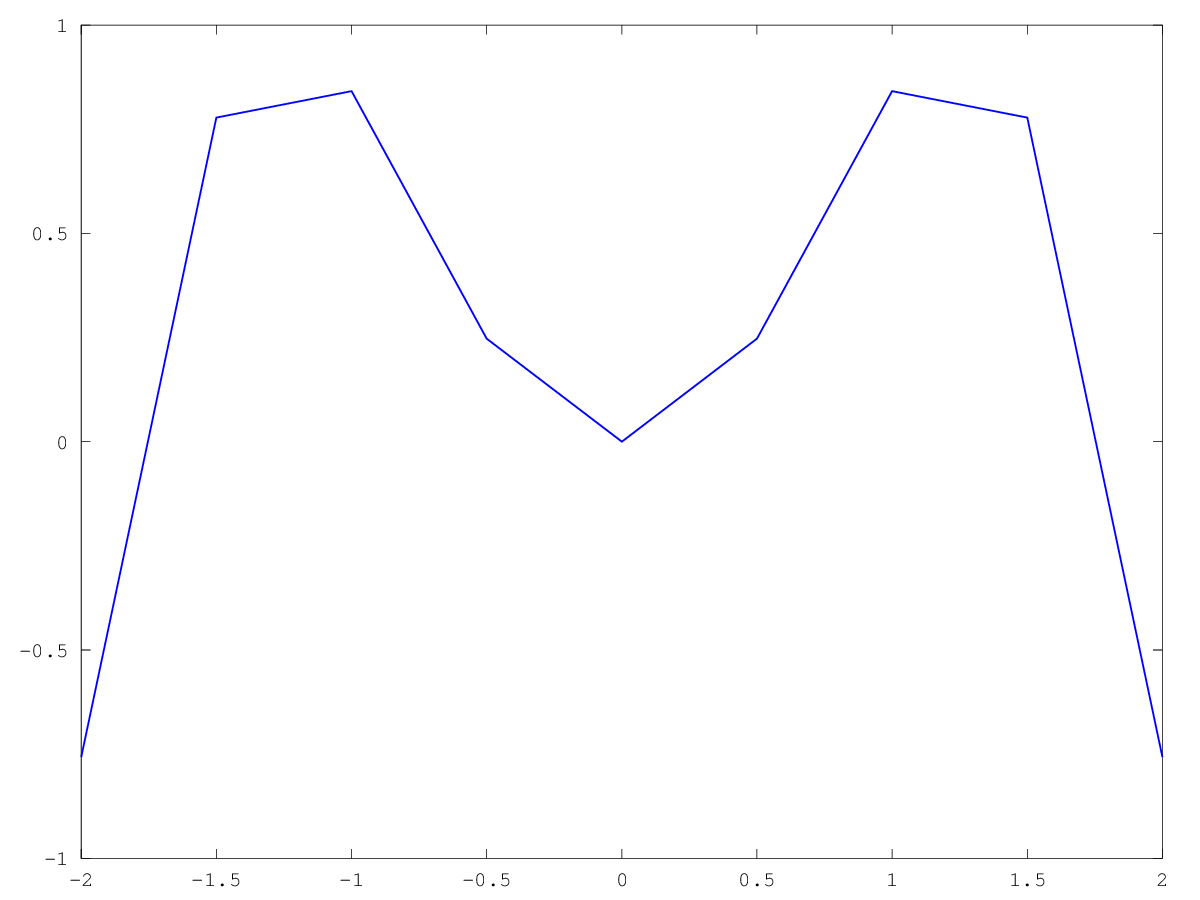
\includegraphics[height=180pt]{figures/coarse.png}
\end{center}
\end{figure}


This is not a good figure, and indeed, we should not at all
be feeling proud at this time. For a relatively `smooth' graph,
we will need to plot a lot more values. How about \texttt{x}
with an interval of \texttt{0.1} instead of \texttt{0.5}?

\begin{minted}[bgcolor=bg]{octave}
    >> x = [-2 -1.9 -1.8 -1.7 -1.6 -1.5  --
    >> % No.
\end{minted}

Of course, there is a smarter way to do this. Matlab 
provides a very neat construct to generate series with
evenly spaced values:

\begin{minted}[bgcolor=bg]{octave}
    
    >> x = -2:0.1:2;  % From -2 to +2 in steps of 0.1
    >> disp(x)        % See how it looks!
    >> y = sin(x.^2);
    >> plot(x,y);

\end{minted}

\begin{figure}[h]
\begin{center}
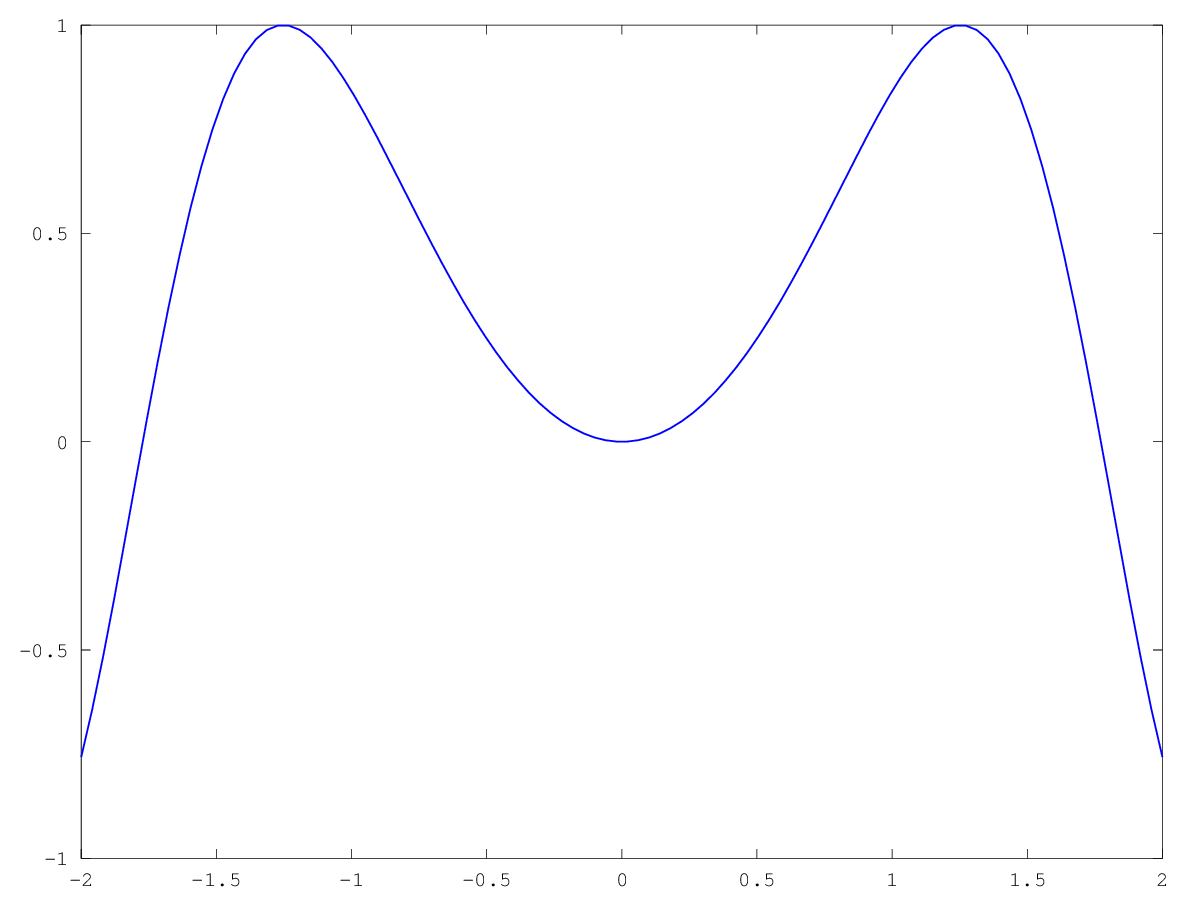
\includegraphics[height=180pt]{figures/fine.png}
\end{center}
\end{figure}

\section*{Exercise: }

Now you know how to spawn a series of values and evaluate and graph a 
function. Let's do something cool with functions. Of course, some functions 
are more interesting than others. For instance, consider this one:

\begin{center}
$y = e^{-0.2t}sin(t)$
\end{center}

This function describes the behaviour of a damped spring with time.
See \url{http://en.wikipedia.org/wiki/File:Damped_spring.gif}. 

Notice that the paramter $t$ is a measure of \emph{time} in say, seconds. 
Graph $y$ for $t$ from 0 to 30 seconds. Convince yourself that this figure 
does indeed describe the behaviour of a damped spring.

Simply graphing a function can yield a surprising amount of information.
For instance, with the figure you generated, you should be able to:


\begin{itemize}
\item{Find the maximum amplitude (the first peak)}
\item{Find the time at which the 3rd peak is reached}
\item{Find the time at which the amplitude falls below some threshold 
(we can consider the oscillation to have stopped after this threshold is
reached)}

\end{itemize}



\end{document}

